\documentclass[preprint,12pt,a4paper]{elsarticle}

\usepackage{amssymb}
\usepackage{amsmath}
\usepackage{graphicx}
\usepackage{booktabs}
\usepackage{hyperref}
\usepackage{listings}
\usepackage{xcolor}
\usepackage{tikz}
\usepackage{multirow}
\usepackage{placeins}
\usepackage{array}
\usepackage{tabularx}
\usepackage{microtype}
\usetikzlibrary{arrows.meta,positioning,shapes.geometric,fit,backgrounds,calc}

% --- Revision tracking: accepted edits are uncoloured;
%     earlier supervisor edits remain in blue and green,
%     orange edits are from the v13 round,
%     RED edits are new in v18 (consistency and repetition pass). ---
\definecolor{RevisionRed}{RGB}{180,0,0}
\definecolor{RevisionBlue}{RGB}{0,76,153}
\definecolor{RevisionGreen}{RGB}{0,120,60}
\definecolor{RevisionOrange}{RGB}{180,90,0}
\newcommand{\rev}[1]{{#1}}
\newcommand{\revb}[1]{{#1}}
\newcommand{\revg}[1]{{#1}}
\newcommand{\revo}[1]{{#1}}
\newcommand{\revr}[1]{{#1}}

\lstset{
  language=Python,
  basicstyle=\ttfamily\footnotesize,
  keywordstyle=\color{blue},
  commentstyle=\color{gray},
  stringstyle=\color{red!70!black},
  frame=single,
  breaklines=true,
  captionpos=b,
}

\emergencystretch=2em

\journal{SoftwareX}

\begin{document}

\begin{frontmatter}

\title{\texttt{weatherisk}: A Python Package for Spatial Clustering
  of Climate Extremes via Max-Stable Processes}

\author[awi,uni]{Widad Kchikach\corref{cor1}}
\ead{widad.kchikach@awi.de}
\cortext[cor1]{Corresponding author}

\author[uni]{Thorsten Dickhaus}
\author[awi,uni]{Gerrit Lohmann}

\address[awi]{Alfred Wegener Institute Helmholtz Centre for Polar
  and Marine Research, Bremerhaven, Germany}
\address[uni]{University of Bremen, Bremen, Germany}

\begin{abstract}
We present \texttt{weatherisk}, an open-source Python package for
identifying regions of homogeneous extremal dependence in gridded
climate-model output. The package implements a
complete analysis pipeline: seasonal-trend decomposition (STL) removes
long-term trends from raw monthly fields; annual block maxima are
extracted and fitted with generalised extreme-value (GEV)
distributions; marginals are transformed to unit Fr\'{e}chet
scale---the standard heavy-tailed reference form required by max-stable
models---and local spatial-dependence parameters are estimated before
grid cells are partitioned into coherent regions. Two clustering
schemes are supported---Local Estimates Clustering (LEC) and Extremal
Dependence Clustering (EDC)---each validated at every pipeline stage
against an established R reference implementation to ensure numerical
fidelity. We demonstrate \texttt{weatherisk} on a global-precipitation
case study using the AWI-ESM-1-1-LR model (T63 grid, $192\times96$
cells, 1850--2005), executed on the AWI \emph{albedo}
high-performance cluster, reproducing a published cluster map entirely
in Python. The result is a reproducible, scalable framework for
spatial-extremes analysis, suited equally to synthetic benchmarks and
publication-scale climate-model output.
\end{abstract}

\begin{keyword}
spatial extremes \sep max-stable process \sep
spatial clustering \sep extremal dependence \sep Python
\end{keyword}

\end{frontmatter}

%% ============================================================
\section*{Metadata}
\label{sec:metadata}
%% ============================================================

Table~\ref{tab:metadata} summarises the mandatory software metadata
for the current release of \texttt{weatherisk}.

\begin{table}[!h]
\small
\begin{tabularx}{\textwidth}{|l|>{\raggedright\arraybackslash}p{4.9cm}|>{\raggedright\arraybackslash}X|}
\hline
\textbf{Nr.} & \textbf{Code metadata description} & \textbf{Metadata} \\
\hline
C1 & Current code version & v0.1.0 \\
\hline
C2 & Permanent link to code/repository &
  \url{https://github.com/wkchikach99-byte/weatherisk} \\
\hline
C3 & Permanent link to Reproducible Capsule &
  \url{https://doi.org/10.5281/zenodo.XXXXXXX} (to be assigned on first GitHub release) \\
\hline
C4 & Legal Code License & MIT \\
\hline
C5 & Code versioning system used & git \\
\hline
C6 & Software code languages, tools, and services used &
  Python~3.10+; optional Rust backend; R (validation); SLURM \\
\hline
C7 & Compilation requirements, operating environments
  \& dependencies &
  Python~$\geq$3.10; NumPy; SciPy; pandas; matplotlib;
  Click; xarray; netCDF4; scikit-learn; Cartopy; h5py;
  statsmodels; optional pytest/ruff/mypy for development \\
\hline
C8 & Link to developer documentation &
  \url{https://github.com/wkchikach99-byte/weatherisk} \\
\hline
C9 & Support email for questions & widad.kchikach@awi.de \\
\hline
\end{tabularx}
\caption{Code metadata (mandatory).}
\label{tab:metadata}
\end{table}


%% ============================================================
\section{Motivation and significance}
\label{sec:motivation}
%% ============================================================

Extreme weather events such as heavy precipitation or heat waves
rarely act on a single location; they typically unfold across broad
regions at once~[1]. Understanding \emph{where} such events tend to
co-occur matters enormously for regional risk assessment, reinsurance,
and infrastructure planning. Ignoring the spatial footprint of
extremes can lead to a serious underestimate of aggregate losses.

\revg{While mean climate trends carry important information,
socioeconomic impacts are driven disproportionately by extreme events
rather than by shifts in average conditions~[1]. Infrastructure
failures, crop losses, and flood damage are governed by tail
probabilities (the chances of exceeding a rarely reached, very high
threshold)---not by means---of precipitation and temperature
distributions. Getting the tail behaviour and its spatial dependence
structure right is therefore central to any serious risk
quantification.}

\revg{Extremes also behave differently from everyday climate
variability: they show non-Gaussian distributions, heavy
tails (where extreme values occur far more often than a bell-curve
distribution would predict), and asymptotic dependence---also called
\emph{extremal dependence} throughout this paper---none of which standard
covariance-based techniques adequately represent~[2]. Extreme
value theory (EVT) provides the rigorous mathematical framework
for this regime. A central concept in EVT is the \emph{block
maximum}: the single largest observed value within a fixed time
window---here, one calendar year. Annual block maxima follow a
\emph{generalised extreme-value} (GEV) distribution, a
three-parameter family that characterises how the magnitude of the
largest events grows with record length. Crucially, this result
holds regardless of the underlying data distribution, which is why
EVT methods remain valid even over the centuries-long simulation
periods typical of climate modelling~[2,3]. Capturing these complex
spatial patterns requires both a statistically sound framework and
software that can handle the associated computational burden---the
dual motivation for the present work.}

\emph{Max-stable processes} are the standard framework for
modelling joint tail behaviour across space~[2,3].
Following Contzen et al.~[4], fitting these models at each location
yields anisotropy parameters that capture the strength and
directional orientation of local spatial dependence.
Grid cells with similar parameter estimates can then be grouped
into \emph{clusters}---geographically connected regions in which
the extremal dependence structure is approximately uniform.

An R-based pipeline that implements this workflow was developed
by Contzen et al.~[4]. It simulates max-stable processes,
estimates local anisotropy parameters via pairwise composite
likelihood~[3] \revr{(see Section~\ref{sec:architecture} for the
technical details)}, computes a pairwise dissimilarity score between
all grid cells based on the geometric overlap of their fitted
anisotropy ellipses, and partitions cells by hierarchical clustering. In practice,
however, the implementation is fragmented across independent
R scripts tied together by SLURM shell files, which makes
installation, testing, and extension unnecessarily difficult.
\rev{This limitation becomes particularly acute in climate-model
applications, where extremes are, by definition, rare, and stable
statistical inference requires long time series---decades or
centuries. Modern coupled models such as AWI-ESM-1-1-LR produce
monthly output on global grids (e.g.\ T63, $192 \times 96 = 18{,}432$ cells) spanning hundreds of simulated years.  Processing
these heavy NetCDF archives before any clustering can begin involves
detrending, block-maxima extraction, GEV marginal fitting (estimating
a separate GEV distribution independently at each grid cell), and
Fr\'{e}chet transformation at every grid cell.  Scientific software
for this problem therefore has to do more than implement the
mathematics: it must also provide a reproducible preprocessing chain,
checkpoint/restart support for long-running jobs, and numerically
efficient kernels that scale from laptops to high-performance
computing facilities.}

\texttt{weatherisk} solves this problem by re-implementing the full
pipeline in a single Python package that can be installed with
\texttt{pip install}.  It faithfully reproduces every step of the
original R code at reduced and controlled scales and adds several
practical features:
\begin{itemize}
\item \rev{a complete preprocessing chain for climate-model output:
  STL (Seasonal-Trend decomposition using Loess) detrending, annual
  block-maxima extraction, GEV fitting, and Fr\'{e}chet transformation
  (a probability-integral step that maps each grid cell's fitted GEV
  values to a common unit-Fr\'{e}chet scale required by the max-stable
  model)};
\item \rev{checkpoint/restart support and scalable execution
  strategies for heavy CMIP6\revo{ (Coupled Model Intercomparison
  Project Phase~6)}-style workloads on high-performance
  computing (HPC) infrastructure}; and
\item \rev{a 196-test validation suite, including 30~end-to-end
  CMIP6 parity tests (Section~\ref{sec:validation})}.
\end{itemize}

\rev{To demonstrate the software on a publication-level workload, we
include a \revb{Python-based revisit of the Figure~9 case study} from Contzen et al.~[4] on the
AWI-ESM-1-1-LR historical precipitation dataset and provide a
systematic model-validation analysis (Section~\ref{sec:validation})
documenting the precision of every pipeline stage against the original
R implementation.}

Existing Python packages do support parts of the extreme-value workflow.
For example, \texttt{pyextremes}~[5] and
\texttt{scikit-extremes}\footnote{\url{https://github.com/kikocorreoso/scikit-extremes}}
focus on univariate extreme-value analysis, while the R package
\texttt{SpatialExtremes}~[6] provides max-stable simulation.
However, to our knowledge, no existing Python package offers the
integrated spatial-extremes workflow implemented here: max-stable
simulation, local composite-likelihood estimation, and ellipse-based
spatial clustering of extremes in one package.

%% ============================================================
\section{Software description}
\label{sec:description}
%% ============================================================

\subsection{Software architecture}
\label{sec:architecture}

\texttt{weatherisk} is a pip-installable Python package organised
into 18~modules and a CLI entry point.  Figure~\ref{fig:workflow}
shows the overall workflow.

\rev{The processing pipeline consists of seven stages. The first
stage contains three sub-steps that together convert raw climate-model
output into the standardised representation required by the
subsequent statistical analysis:}

\begin{enumerate}
\item \textbf{\rev{Preprocessing.}}
  \begin{enumerate}
  \item[\textbf{(a)}] \textbf{\rev{STL decomposition (detrending).}}
    \rev{Raw monthly precipitation fields are decomposed using the
    STL method of Cleveland et al.~[10] with \texttt{s.window =
    ``periodic''} and \texttt{robust = TRUE}.  The trend component is
    subtracted, retaining the seasonal cycle and residuals. This step
    isolates the stationary signal needed for extreme-value
    modelling. Both a native Python implementation and an optional
    R-subprocess path (for exact cross-validation against the
    original R workflow) are provided.}
  \item[\textbf{(b)}] \textbf{\rev{Annual block-maxima extraction.}}
    \rev{From the detrended monthly series, the annual maximum
    precipitation value is extracted for each grid cell, keeping
    only years with all 12 months present. The result is an
    $(n_{\text{years}} \times n_{\text{cells}})$ matrix of annual
    extremes that feeds the marginal fitting step. Taking the
    annual maximum is the standard ``block maxima'' approach of
    classical EVT~[2].}
  \item[\textbf{(c)}] \textbf{\rev{GEV fitting and Fr\'{e}chet
    transformation.}}
    \rev{A GEV distribution is fitted independently at each grid cell
    by maximum likelihood. Before fitting, cells that are entirely
    missing or have near-zero variance are excluded; isolated missing
    values in the remaining cells are replaced by the cell-wise mean.
    Any cell that still yields non-finite GEV or Fr\'{e}chet values
    after fitting is dropped. In the full AWI-ESM-1-1-LR run, all
    $192 \times 96 = 18{,}432$ cells passed this screen. The fitted
    GEV at each cell is then used to apply the probability integral
    transform: each annual maximum is mapped through its own GEV
    cumulative distribution function, producing a value on the
    unit Fr\'{e}chet scale (the common marginal form required by
    max-stable models, as described in Section~\ref{sec:motivation}).
    \revr{This puts all cells on an equal footing before spatial
    dependence is estimated: what remains captures where extremes
    co-occur, not how large they are at any individual site.}
    Values are clipped to $[0.05,\, n_{\text{years}}^{2}]$ to
    suppress numerical artefacts at the tails.}
  \end{enumerate}
\item \textbf{Simulation} (for validation on synthetic data).
  Synthetic max-stable random fields with
  user-specified spatially varying anisotropy are generated on a
  regular grid following the spectral construction of
  Schlather~[7]. These fields serve as controlled test cases whose
  true parameters are known by construction.
\item \textbf{Local estimation.}
  For each grid cell, we estimate the three local anisotropy
  parameters---semi-axis lengths $a$ and $b$ (controlling the range
  and degree of directional asymmetry of spatial dependence) and a
  rotation angle $\gamma$ (the principal direction of dependence)---by
  maximising a pairwise composite likelihood~[3,4]\revr{, which sums
  log-likelihood contributions over neighbouring grid-cell pairs;
  this avoids fitting the full joint spatial distribution at once and
  makes estimation computationally feasible on large grids.} The
  optimisation runs over all neighbouring pairs within grid-point
  distance $\varepsilon$ (default $\varepsilon=5$).
  \rev{Neighbours are enumerated in a fixed stencil order
  (x-offset varies fastest) matching the R reference, and at least
  three valid neighbours are required; cells with fewer than five
  valid pairs receive default estimates $(a,b,\gamma) = (1,0,0)$.
  A multi-start strategy with five random restarts (seed = 42)
  mitigates sensitivity to local optima~[4]. Fr\'{e}chet values
  are normalised to 11 decimal places before optimisation to
  ensure numerical parity with the R workflow at the precision
  boundary.}
\item \textbf{\rev{Spatial smoothing.}}
  \rev{The raw estimates $(a_i, b_i, \gamma_i)$ are smoothed by a
  moving average over grid cells within a smoothing radius (default
  2.0 in grid-point units).  Angular wrapping is applied to the
  rotation angle $\gamma$ to account for its directional
  periodicity ($+90^{\circ} \equiv -90^{\circ}$).}
\item \textbf{Clustering.}
  From the smoothed parameter estimates, we assemble a pairwise
  dissimilarity matrix and apply average-linkage hierarchical
  agglomerative clustering~[4] to group grid cells into regions.
  The number of clusters $k$ is set automatically by applying a
  quantile threshold (default: 30\textsuperscript{th} percentile)
  to the dendrogram merge heights, following Contzen et al.~[4].
  Two dissimilarity measures are available:
  \begin{itemize}
  \item \textbf{LEC} (Local Estimates Clustering~[4]; ellipse-overlap
    dissimilarity $D_2$): Jaccard-like overlap of the anisotropy
    ellipses\revo{ (a ratio of intersection to union area, ranging
    from 0 for non-overlapping to 1 for identical ellipses; here
    used as a geometrically interpretable dissimilarity $1 - \text{overlap}$)}.
    \revr{Each grid cell's fitted parameters $(a, b, \gamma)$ define
    an ellipse in 2D space. Two cells whose ellipses overlap strongly
    have a similar dependence geometry, so high overlap means low
    dissimilarity. The ratio $D_2$ was introduced by Contzen
    et al.~[4] as a geometrically clear way to measure this.}
  \item \textbf{EDC} (Extremal Dependence Clustering~[4]; madogram-based
    dissimilarity $D_1$, following Cooley et al.~[9] and Saunders et al.~[8]):
    \revo{The madogram is a rank-based summary of extremal
    dependence: computed from order statistics without parametric
    assumptions, it maps onto pairwise extremal coefficients that
    range from 1 (complete dependence: extreme events at the two
    sites always co-occur) to 2 (independence), with intermediate
    values reflecting partial co-occurrence~[9].  Contzen et al.~[4]
    adopt this approach alongside the ellipse method, providing an
    alternative non-parametric dissimilarity $D_1$ for
    dependence-based regionalisation.}
  \end{itemize}
\item \textbf{\rev{In-cluster re-estimation.}}
  \rev{Within each cluster, the dependence parameters are
  re-estimated using all data from the cluster's grid cells via
  global pairwise composite-likelihood maximum-likelihood estimation
  (MLE; distance cutoff: $4.0
  \times$ neighbour radius, 3 restarts per cluster). The
  goodness-of-fit of each method is assessed.}
\end{enumerate}

\begin{figure}[ht]
\centering
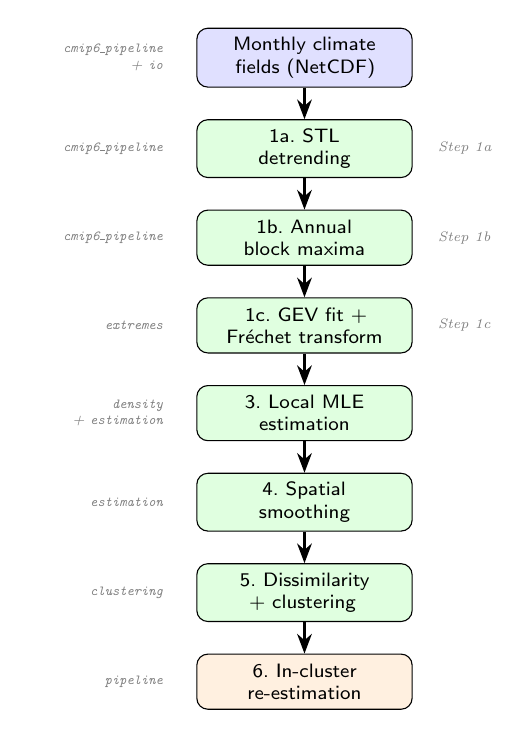
\begin{tikzpicture}[
  box/.style={draw, rounded corners=4pt, minimum width=2.6cm,
    minimum height=0.7cm, font=\sffamily\scriptsize,
    align=center, text width=2.5cm},
  data/.style={box, fill=blue!12},
  proc/.style={box, fill=green!12},
  outbox/.style={box, fill=orange!12},
  arr/.style={-{Stealth[length=2.5mm]}, thick},
  note/.style={font=\itshape\tiny, text=gray},
  node distance=0.4cm,
]

\node[data] (raw) {Monthly climate\\fields (NetCDF)};

\node[proc, below=of raw] (stl)
  {\rev{1a.\ STL\\detrending}};
\node[proc, below=of stl] (bm)
  {\rev{1b.\ Annual\\block maxima}};
\node[proc, below=of bm] (frech)
  {\rev{1c.\ GEV fit +\\Fr\'{e}chet transform}};
\node[proc, below=of frech] (mle)
  {3.\ Local MLE\\estimation};
\node[proc, below=of mle] (smooth)
  {4.\ Spatial\\smoothing};
\node[proc, below=of smooth] (clust)
  {5.\ Dissimilarity\\+ clustering};
\node[outbox, below=of clust] (out)
  {6.\ In-cluster\\re-estimation};

\draw[arr] (raw) -- (stl);
\draw[arr] (stl) -- (bm);
\draw[arr] (bm) -- (frech);
\draw[arr] (frech) -- (mle);
\draw[arr] (mle) -- (smooth);
\draw[arr] (smooth) -- (clust);
\draw[arr] (clust) -- (out);

% Module names on the left
\node[note, left=0.3cm of raw, text width=1.6cm, align=right]
  {\texttt{cmip6\_pipeline}\\+ \texttt{io}};
\node[note, left=0.3cm of stl, text width=1.6cm, align=right]
  {\rev{\texttt{cmip6\_pipeline}}};
\node[note, left=0.3cm of bm, text width=1.6cm, align=right]
  {\rev{\texttt{cmip6\_pipeline}}};
\node[note, left=0.3cm of frech, text width=1.6cm, align=right]
  {\texttt{extremes}};
\node[note, left=0.3cm of mle, text width=1.6cm, align=right]
  {\texttt{density}\\+ \texttt{estimation}};
\node[note, left=0.3cm of smooth, text width=1.6cm, align=right]
  {\texttt{estimation}};
\node[note, left=0.3cm of clust, text width=1.6cm, align=right]
  {\texttt{clustering}};
\node[note, left=0.3cm of out, text width=1.6cm, align=right]
  {\texttt{pipeline}};

% Stage labels on the right
\node[note, right=0.2cm of stl] {Step 1a};
\node[note, right=0.2cm of bm] {Step 1b};
\node[note, right=0.2cm of frech] {Step 1c};

\end{tikzpicture}
\caption{\rev{Processing pipeline of \texttt{weatherisk}. Stage~1
  (a--c) is the preprocessing chain added for climate-model data;
  stages~3--6 implement the core statistical methodology of Contzen
  et al.~[4]. Module names are shown on the left.}}
\label{fig:workflow}
\end{figure}

\subsection{Software functionalities}
\label{sec:functionalities}

Section~\ref{sec:architecture} describes the end-to-end workflow.
This subsection instead summarises the main software components and
their roles within the package.

\paragraph{Covariance modelling (\texttt{covariance})}
This module implements the anisotropic covariance functions used by
the max-stable dependence model, including stationary and
non-stationary formulations and the conversion between covariance and
extremal-coefficient representations.

\paragraph{Simulation (\texttt{simulation})}
The simulation module generates synthetic max-stable fields with
spatially varying anisotropy. These synthetic datasets are used for
method development, controlled validation experiments, and regression
tests against known parameter fields.

\paragraph{Preprocessing and extremes (\texttt{cmip6\_pipeline}, \texttt{netcdf}, \texttt{extremes})}
These components handle gridded climate-model input, including NetCDF
loading, STL detrending of monthly series, annual block-maxima
extraction, GEV fitting, and transformation to unit Fr\'{e}chet
margins. Together they provide the climate-data preprocessing chain
required before spatial dependence can be estimated.

\paragraph{Estimation (\texttt{density}, \texttt{estimation})}
These modules implement pairwise composite-likelihood estimation of
the local anisotropy parameters $(a,b,\gamma)$, the subsequent spatial
smoothing step, and the in-cluster re-estimation routines used after
clustering. They also contain the numerical safeguards needed for
stable optimisation on large grids.

\paragraph{Clustering (\texttt{clustering})}
This module provides the two regionalisation methods implemented in
\texttt{weatherisk}: LEC (Local Estimates Clustering), based on
ellipse-overlap dissimilarity, and EDC (Extremal Dependence
Clustering), based on madogram-derived extremal dependence. It also provides
the hierarchical clustering utilities that convert these
dissimilarities into region labels.

\paragraph{Scalability and execution (\texttt{scalable}, \texttt{cli})}
These components support large production runs through parallel
execution, checkpoint/restart handling, and command-line entry points
for the main workflows. They are designed to make the same code base
usable both for local experiments and for HPC-scale Figure~9
\revb{case-study analysis}.

\paragraph{Plotting and outputs (\texttt{plotting}, \texttt{map\_plotting})}
The plotting modules generate diagnostic figures, synthetic-study
visualisations, and the publication-style cluster maps used in the CPC
and CMIP6 workflows. They provide the final user-facing outputs of the
pipeline in addition to the saved numerical arrays.

\subsection{Computational performance}
\label{sec:performance}

The dominant costs are the $O(n^2)$ pairwise dissimilarity matrix and
per-cell local MLE optimisation.
\texttt{weatherisk} reduces both in four ways:

\begin{enumerate}
\item \textbf{Batch covariance.}
  All $n^2$ entries are evaluated in a single vectorised NumPy call;
  $2\times 2$ matrix inverses use the analytic closed-form formula.

\item \textbf{Pre-drawn ellipse overlap (LEC).}
  Each fitted ellipse is rasterised once; pairwise overlap areas
  are computed with bitwise operations over batches of 256 pairs.

\item \textbf{Fast pairwise distance (EDC).}
  \texttt{scipy.spatial.distance.\allowbreak{}cdist} evaluates all
  pairwise rank-based distances in a single compiled-C call.

\item \textbf{Parallel local estimation.}
  Per-cell MLE tasks are distributed via Python's
  \texttt{multiprocessing}; shared data is loaded once per worker.
\end{enumerate}

On the same 6$\times$6 synthetic input, the Python pipeline
completed in 17.9\,s compared with 43.9\,s for the original
R~implementation---a 2.5$\times$ speed-up on an identical workload.
The full AWI-ESM-1-1-LR T63 grid (18{,}432 cells, 156~years) was
run on the AWI \emph{albedo} HPC cluster using 16~parallel workers,
completing in approximately 4~hours with peak memory below 2\,GiB;
SLURM scripts and setup are provided under \texttt{hpc/}.

\paragraph{Command-line interface (\texttt{cli}).}
A single entry point exposes the main pipeline flows:
\begin{lstlisting}[numbers=none]
$ weatherisk validate --params stripes \
    --resolution 10 --n-sim 20 --seed 42
$ weatherisk maps --variable precip
\end{lstlisting}

%% ============================================================
\section{Illustrative examples}
\label{sec:examples}
%% ============================================================

We demonstrate \texttt{weatherisk} with \rev{two} examples: one on
synthetic data \rev{and one \revb{Python-based revisit of Figure~9 from Contzen}
et al.~[4] on the AWI-ESM-1-1-LR climate model}.

\subsection{Example~1: Synthetic validation}
\label{sec:ex-synthetic}

In this example, we simulate max-stable data on a 51$\times$51 grid
where the semi-major axis $b$ increases linearly from left to right,
creating vertical ``stripe'' regions.  The pipeline should recover
these stripes from the simulated data alone.

\begin{lstlisting}[caption={Running the stripes validation.},
  label=lst:validate]
from weatherisk.parameters import get_preset
from weatherisk.pipeline import run_pipeline

result = run_pipeline(
    resolution=51, n_sim=20,
    preset="stripes", seed=42,
)
\end{lstlisting}

Figure~\ref{fig:stripes} shows the result.  Panel~(a) displays the
EDC clusters ($k_{\text{edc}} = 7$), panel~(b) the LEC clusters
($k_{\text{lec}} = 5$), and panel~(c) the true parameter field.
The true semi-major axis~$b$ increases smoothly from left to right
(panel~c), producing a continuous gradient from dark blue ($b
\approx 0$) on the left to light shading ($b \approx 5$) on the
right.  The EDC method (panel~a) uses seven clusters and captures
the overall left-to-right trend, but its boundaries are irregular:
some clusters extend horizontally across the domain, and the
transitions between adjacent regions do not follow the vertical
orientation of the true gradient.  The LEC method (panel~b), by
contrast, uses only five clusters yet produces boundaries that are
predominantly vertical, closely tracking the true transitions in
the parameter field.  The estimated within-cluster~$b$ values in
the LEC map also progress monotonically from dark to light,
mirroring the ground truth more faithfully than the EDC partition.
This controlled experiment illustrates that the Python
implementation correctly recovers the known spatial structure,
consistent with the methodology of Contzen et al.~[4].  Formal
verification of numerical equivalence with the original R code
is provided by the automated cross-validation tests described
in Section~\ref{sec:validation}.

\begin{figure}[!htbp]
\centering

\includegraphics[width=0.95\textwidth]{figures/fig3_regenerated.png}
\caption{Synthetic validation on the ``stripes'' preset
  ($k_{\text{edc}} = 7$, $k_{\text{lec}} = 5$).
  (a)~EDC clusters coloured by estimated semi-major axis~$b$;
  (b)~LEC clusters coloured by estimated~$b$;
  (c)~true parameter field showing a smooth left-to-right
  gradient in~$b$ from 0 to~5.
  The LEC method recovers sharper, vertically aligned boundaries
  that closely match the ground truth, while the EDC method
  produces more irregular, horizontally extended partitions.}
\label{fig:stripes}
\end{figure}

\FloatBarrier

\rev{\subsection{Example~2: \revb{Revisiting the Figure~9 case study} --- AWI-ESM-1-1-LR
  global precipitation}}
\label{sec:ex-fig9}

\rev{To demonstrate the software on the same data used in the original
publication, we \revb{revisit the Figure~9 analysis} of Contzen et al.~[4].  The
experiment uses monthly precipitation from the AWI-ESM-1-1-LR
historical simulation (T63 grid, $192 \times 96$ cells, r1i1p1f1,
years 1850--2005) with the parameter settings listed in
Table~\ref{tab:fig9-params}, following Section~5 of~[4]:}

\begin{table}[ht]
\centering
\begin{tabular}{ll}
\toprule
\textbf{Parameter} & \textbf{Value} \\
\midrule
Degrees of freedom $\nu$ & 5 \\
Covariance exponent $\alpha$ & 1 \\
Neighbour radius $\varepsilon$ & 5 (grid-point units) \\
Clustering quantile threshold & 30\textsuperscript{th} percentile \\
Model / experiment & AWI-ESM-1-1-LR / historical \\
Grid / resolution & T63 ($192 \times 96$) \\
Period & 1850--2005 (156~years) \\
\bottomrule
\end{tabular}
\caption{Parameter settings used for the Figure~9 \revb{case-study analysis},
  following Section~5 of Contzen et al.~[4]. \revo{The degrees of
  freedom $\nu$ and covariance exponent $\alpha$ are parameters of
  the Schlather max-stable dependence model~[7]: $\nu$ controls
  how quickly dependence decays with distance (higher $\nu$ gives
  weaker long-range dependence), and $\alpha \in (0,\,2]$
  controls the smoothness of the simulated fields.}}
\label{tab:fig9-params}
\end{table}

\rev{The full seven-stage pipeline (Section~\ref{sec:architecture}) was
executed on the AWI \emph{albedo} HPC cluster (16~CPU cores;
SLURM scripts in \texttt{hpc/}). The command-line invocation is:}

\begin{lstlisting}[caption={\revb{Running the Figure~9 case study on HPC}.},
  label=lst:fig9, numbers=none]
$ python scripts/reproduce_fig9.py \
    --data-dir /path/to/AWI-ESM-1-1-LR/pr/ \
    --workers 16  --output-dir output/cmip6_fig9 \
    --dpi 300
\end{lstlisting}

\rev{Figure~\ref{fig:fig9} shows the result, and
Table~\ref{tab:fig9-counts} compares the resulting cluster counts with
those reported by Contzen et al.~[4]:}

\begin{table}[ht]
\centering
\begin{tabular}{lcc}
\toprule
\textbf{Method} & \textbf{Contzen et al.~[4]} &
  \textbf{\texttt{weatherisk}} \\
\midrule
EDC ($k_{\text{edc}}$) & 104 & 142 \\
LEC ($k_{\text{lec}}$) & 24 & 21 \\
\bottomrule
\end{tabular}
\caption{Cluster counts reported in Contzen et al.~[4] and obtained
  with \texttt{weatherisk} for the full Figure~9 \revb{case-study run}.}
\label{tab:fig9-counts}
\end{table}

\rev{The LEC result ($k_{\text{lec}} = 21$ vs.\ 24) is close; the
remaining difference is consistent with the level of variation
expected from differences in preprocessing conventions and from the
flat optimisation landscape of the composite-likelihood surface at
this scale. In particular, the Python workflow makes explicit choices
about detrending, GEV fitting, partial-missing-value handling, and
post-fit removal of non-finite cells that are not described in the
same operational detail in Contzen et al.~[4]. The EDC
discrepancy is larger ($k_{\text{edc}} = 142$ vs.\ 104); we
attribute this primarily to differences in preprocessing and missing-
data handling---details that are not fully specified in the published paper
---rather than to any algorithmic deviation. Our coding and testing
work shows that, on controlled mini-pipeline inputs, the Python
implementation reproduces the R reference cluster counts exactly for
both methods (Section~\ref{sec:validation}). This supports the
correctness of the methodology itself. At the full Figure~9 scale,
the most plausible explanation is therefore not that the method is
wrong, but that the published workflow leaves some preprocessing
choices implicit. A separate point concerns LEC only: we identified a
logical indexing issue in the original R ellipse-dissimilarity code.
More precisely, in the R function \texttt{calc\_distance\_ellipses}
(\texttt{r\_code/functions.R}, line 515 in the repository version used
here), the empty-ellipse branch inside the nested loop over grid-cell
indices \texttt{i} and \texttt{j} writes \texttt{dist\_matrix[j] = 1}
rather than \texttt{dist\_matrix[i,j] <- 1}. Because \texttt{dist\_matrix[j]}
uses linear indexing in R, the routine still executes and returns an
output map, but some LEC dissimilarity values can be placed in
incorrect matrix positions. This issue may contribute to the small
remaining LEC difference, but it does not explain the larger EDC
difference, which is more naturally linked to preprocessing and
valid-cell-mask differences.}

\FloatBarrier
\begin{figure}[!htbp]
\centering

\includegraphics[width=0.95\textwidth]{figures/fig9_combined_42260990.png}
\caption{\rev{\revb{Python-based revisit of Figure~9} from Contzen et al.~[4] using
  \texttt{weatherisk}. Left: EDC clusters ($k_{\text{edc}} = 142$).
  Right: LEC clusters ($k_{\text{lec}} = 21$). The experiment uses
  AWI-ESM-1-1-LR historical precipitation on the T63 grid
  (1850--2005) with $\nu = 5$, $\alpha = 1$, $\varepsilon = 5$,
  and 30\% quantile threshold. The LEC panel shows spatially
  coherent regions consistent with the published Figure~9; the
  EDC panel captures the expected global heterogeneity of
  extremal dependence.}}
\label{fig:fig9}
\end{figure}

\FloatBarrier


%% ============================================================
\rev{\section{Model validation}
\label{sec:validation}}
%% ============================================================

\rev{We verify \texttt{weatherisk} against the original R implementation
of Contzen et al.~[4] at three complementary levels
(Table~\ref{tab:validation}).
\textbf{Level~1 (40 tests):} each mathematical kernel is tested
against R reference values; all pass with relative errors
$\leq 10^{-10}$, after resolving cross-language differences in
matrix storage order (Fortran vs.\ C), angular periodicity of
rotation angles, and likelihood normalisation conventions.
\textbf{Level~2 (30 tests):} a mini AWI-ESM-1-1-LR subset
($5{\times}5$ grid, 20~years) is processed through the full
seven-stage pipeline in both Python and R;
Table~\ref{tab:pipeline-parity} lists per-stage agreement, and
both EDC and LEC produce identical cluster counts on this
controlled input.  At full scale, counts differ from Contzen
et al.\ ($k_{\text{lec}}=21$ vs.\ 24; $k_{\text{edc}}=142$
vs.\ 104), which we attribute to undocumented preprocessing
choices and a known linear-index assignment in the original R
ellipse-dissimilarity routine (\texttt{functions.R}, line~515).
\textbf{Level~3 ($\sim$126 tests):} simulation distributional
properties, checkpoint--resume, serial--parallel equivalence,
and parameter-preset reproducibility.

\begin{table}[!htbp]
\centering
\small
\setlength{\tabcolsep}{5pt}
\begin{tabularx}{\textwidth}{>{\raggedright\arraybackslash}p{4.2cm}c>{\raggedright\arraybackslash}X}
\toprule
\textbf{Pipeline stage} & \textbf{Tests} &
  \textbf{Agreement criterion} \\
\midrule
Detrending (STL) & 2 &
  mean absolute difference $< 0.01$ \\
Annual block-maxima extraction & 1 &
  relative error $< 10^{-10}$ \\
GEV fitting and Fr\'{}echet transform & 1 &
  relative error $< 0.002$ \\
Local parameter estimation & 5 &
  relative error $< 10^{-6}$ \\
Spatial smoothing & 2 &
  relative error $< 10^{-10}$ \\
EDC dissimilarity matrix & 3 &
  relative error $< 10^{-10}$ \\
EDC cluster count and labels & 4 &
  exact \\
LEC cluster count and labels & 4 &
  exact \\
Python--Rust backend equivalence & 3 &
  identical output \\
Pipeline configuration defaults & 5 &
  exact \\
\midrule
\textbf{Total} & \textbf{30} & \\
\bottomrule
\end{tabularx}
\caption{Per-stage agreement between the Python and R
  implementations on a mini AWI-ESM-1-1-LR subset
  (5$\times$5 grid, 20~years).}
\label{tab:pipeline-parity}
\end{table}

\begin{table}[!htbp]
\centering
\small
\setlength{\tabcolsep}{5pt}
\begin{tabularx}{\textwidth}{>{\raggedright\arraybackslash}p{4.3cm}c>{\raggedright\arraybackslash}X}
\toprule
\textbf{Validation layer} & \textbf{Tests} &
  \textbf{Agreement criterion} \\
\midrule
Per-function R parity &
  40 & relative error $\leq 10^{-10}$ \\
CMIP6 end-to-end parity &
  30 & exact cluster count \\
Serial--parallel equivalence &
  5 & identical output \\
Checkpoint integrity &
  4 & correct resume \\
Parameter-preset reproducibility &
  30 & exact \\
Component \& regression &
  $\sim$87 & per-test criteria \\
\midrule
\textbf{Total} & \textbf{196} & \\
\bottomrule
\end{tabularx}
\caption{Summary of the automated validation suite.
  All 196~tests pass in under 5~minutes on a standard laptop.
  The CMIP6 parity tests verify exact cluster-count agreement
  on a mini AWI-ESM-1-1-LR subset.}
\label{tab:validation}
\end{table}}

\FloatBarrier

%% ============================================================
\section{Impact}
\label{sec:impact}
%% ============================================================

\revg{The core output of \texttt{weatherisk} is a small number of
spatially coherent regions, each characterised by a common extremal
dependence structure. Working with these regions rather than
thousands of individual grid cells makes the analysis tractable and
raises concrete applied questions: which areas share a common
extreme-precipitation hazard, how do hazard boundaries shift across
climate states, and where should spatial risk aggregation be drawn
in insurance or infrastructure planning?}

\revo{\texttt{weatherisk} makes this methodology directly accessible
to any researcher working in Python. It packages a previously
fragmented R/Shell/SLURM workflow as a standard, pip-installable
library that requires no manual dependency management beyond a single
\texttt{pip install} command.}

\rev{\paragraph{Reproducibility and correctness.}
The validation suite described in Section~\ref{sec:validation}
provides three layers of assurance: (i)~per-function agreement
with the R reference to $\leq 10^{-10}$ relative error, (ii)~exact
cluster-count reproduction on a controlled CMIP6 subset, and
(iii)~structural tests covering checkpointing, parallelism, and
parameter integrity. All 196~tests pass on every commit via
continuous integration.
A dedicated smoke test script (\texttt{scripts/release\_smoke\_test.sh})
provides a quick end-to-end check: it installs the package in a clean
environment, runs the CLI, and confirms that the core pipeline completes
correctly within about one minute.}

\paragraph{Computational efficiency.}
The vectorisation and parallelisation strategies described in
Section~\ref{sec:performance} yield large practical speed-ups.
On a $21 \times 21$ synthetic grid (441~cells), the EDC
dissimilarity matrix is computed in 0.02\,s, and the full pipeline
including 8-core parallel estimation completes in under 1\,s.
\rev{On the full AWI-ESM-1-1-LR T63 grid (18{,}432 cells,
156~years), the pipeline completed in approximately 4~hours
on 16~cores of the AWI \emph{albedo} high-performance computing
HPC cluster.}

\revg{That quadratic cost remains the fundamental bottleneck. Vectorisation and parallelisation reduce the constant factor, but sparse approximations or graph-based clustering strategies will ultimately be needed for next-generation kilometre-scale models.}

\revg{\revo{One methodological limitation of} the present framework is
its reliance on block maxima\revr{, meaning only the single largest value per year per cell is used, and sub-annual extremes are missed}.
While this choice is theoretically justified within extreme value
theory and aligns naturally with max-stable modelling, future work
could explore peaks-over-threshold (POT) extensions in a spatial
setting~[1] to improve data efficiency while retaining theoretical
consistency.}

\paragraph{New research directions.}
By providing a clean Python API and CLI, \texttt{weatherisk} lowers
the entry barrier for researchers who wish to apply spatial
clustering of extremes to new domains (e.g., wind speed, sea-level
pressure) or different datasets (e.g., ERA5, CMIP6 projections).

\paragraph{Education.}
The step-by-step pipeline design, the comprehensive test suite,
and the documented code examples (Appendix~\ref{app:code}) make
the package a practical resource for practitioners.  A Jupyter
notebook tutorial (\texttt{notebooks/weatherisk\_quickstart.ipynb})
that walks through the full pipeline on synthetic data is included
in the repository.

%% ============================================================
\section{Conclusions}
\label{sec:conclusions}
%% ============================================================

\revo{We have presented \texttt{weatherisk}, a Python package that
implements the complete pipeline for spatial clustering of climate
extremes via max-stable processes. The package covers the full
preprocessing chain---STL detrending, annual block-maxima extraction,
GEV fitting, and Fr\'{e}chet transformation---followed by local
composite-likelihood estimation of anisotropy parameters and
regionalisation using Local Estimates Clustering (LEC) or Extremal
Dependence Clustering (EDC)~[4]. This consolidates a previously
fragmented R/Shell workflow into a single, tested, pip-installable
library.}

\revg{The software has been verified at three complementary levels:
per-function agreement with the historical R implementation of
Contzen et al.~[4] to $\leq 10^{-10}$ relative error,
end-to-end CMIP6 parity on a controlled subset \revb{with exact
cluster counts}, and broader structural and regression testing
covering checkpointing, parallelism, and parameter integrity.
The full Figure~9 \revb{case-study application} on the
AWI-ESM-1-1-LR T63 grid confirms that \texttt{weatherisk} is both
methodologically faithful to the reference implementation and
scalable to publication-level workloads on HPC infrastructure.}

\revg{Together, these checks give confidence that the results are correct and reproducible. The spatial clustering condenses a large
climate field into a compact description of where extremes co-occur---a
result that speaks directly to practical questions in reinsurance,
infrastructure planning, and climate services. Two limits of the current
design should be stated plainly: the block-maxima approach uses only
one value per grid cell per year, so shorter-duration extremes are
not captured; and the quadratic cost of pairwise comparison makes
kilometre-scale grids impractical with the current algorithm.}

\revo{Several directions follow naturally from these boundaries.
Statistically, peaks-over-threshold extensions in a spatial
setting~[1] would improve data efficiency while preserving the
theoretical framework, and sparse or graph-based dissimilarity
approximations would address the quadratic scaling. On the
engineering side, a compiled Rust extension
(\texttt{weatherisk\_core}) built via PyO3 bindings~[17] demonstrated
a $2.8\times$ end-to-end speed-up on synthetic benchmarks, with the
local MLE step as the principal bottleneck; releasing it as a tested,
opt-in backend is the most immediate next step. Looking further
ahead, GPU parallelisation via CuPy~[15] or Numba~[16] offers a
natural path to handling next-generation kilometre-scale Earth system
simulations without changing the underlying statistical framework.}

\revg{\paragraph{Outlook: Digital Earth System Twins.}
High-resolution digital replicas of the Earth system, such as those
produced by the European Destination Earth initiative, require automated
analysis tools operating at the same scale and cadence.
Spatial clustering of extremes fits naturally into such a pipeline,
converting per-cell dependence estimates into a compact, monitorable
set of homogeneous regions that can be passed to impact models.
Future extensions would require incremental cluster updating, linkage
to socio-economic exposure databases, and objective criteria for
detecting structural regime shifts.}

\revg{\texttt{weatherisk} is available under the MIT licence.}

%% ============================================================
\section*{Acknowledgements}
%% ============================================================

The authors thank the Alfred Wegener Institute Helmholtz Centre for
Polar and Marine Research (AWI) for access to the \emph{albedo}
computing cluster, on which the Figure~9 case-study pipeline was
executed. We thank J.~Contzen for making the original R
implementation publicly available and for helpful discussions during
the development of \texttt{weatherisk}.

\paragraph*{Author contributions.}
W.~Kchikach designed and implemented the software, conducted all
numerical experiments, and wrote the first draft of the manuscript.
T.~Dickhaus and G.~Lohmann supervised the work, contributed to the
scientific conception, and revised the manuscript. All authors read
and approved the final version.

\paragraph*{Funding.}
W.~Kchikach is supported by the MarDATA Helmholtz School for Marine
Data Science [grant number --- to be confirmed]. T.~Dickhaus and
G.~Lohmann acknowledge support from [funding source --- to be confirmed].

%% ============================================================
%% APPENDIX
%% ============================================================
\appendix

\section{Key code examples}
\label{app:code}

\subsection{A.1\quad Synthetic validation (Flow~1)}

\begin{lstlisting}[caption={Complete synthetic validation
  workflow.}, label=lst:app-validate]
from weatherisk.parameters import get_preset
from weatherisk.simulation import simulate_non_stat
from weatherisk.grid import make_grid
from weatherisk.estimation import (
    calc_local_estimates,
    smooth_estimates,
    calc_estimates_in_clusters,
)
from weatherisk.clustering import (
    ellipse_dissimilarity,
    cluster_from_dissimilarity,
    saunders_clustering,
)
from weatherisk.plotting import plot_cluster_map

# 1. Load a parameter preset
p = get_preset("stripes")

# 2. Build a grid and simulate data
grid = make_grid(resolution=10)
data = simulate_non_stat(
    p.params, grid, n_sim=20,
    df=p.df, alpha=p.alpha, seed=42,
)

# 3. Estimate local anisotropy parameters
raw_est = calc_local_estimates(
    data, grid, df=p.df, alpha=p.alpha,
)
est = smooth_estimates(raw_est, grid)

# 4. Cluster by ellipse-overlap dissimilarity
D = ellipse_dissimilarity(est, grid)
clusters = cluster_from_dissimilarity(
    D, quantile_threshold=0.3,
)

# 5. Re-estimate within clusters
in_clust = calc_estimates_in_clusters(
    data, clusters, grid,
    df=p.df, alpha=p.alpha,
)

# 6. Plot
fig = plot_cluster_map(clusters, grid)
fig.savefig("lec_clusters.pdf")
\end{lstlisting}

\rev{\subsection{A.2\quad CMIP6 Figure~9 \revb{case-study workflow}}}

\begin{lstlisting}[caption={\revb{Running the Figure~9 case study} on HPC or
  locally.}, label=lst:app-fig9]
# On HPC (albedo SLURM cluster):
$ sbatch hpc/run_fig9_clean.slurm

# Or locally (requires CMIP6 data):
$ python scripts/reproduce_fig9.py \
    --data-dir /path/to/AWI-ESM-1-1-LR/pr/ \
    --workers 8

# Programmatic access:
from weatherisk.cmip6_pipeline import (
    run_cmip6_pipeline,
    CMIP6Config,
)
cfg = CMIP6Config()  # paper defaults
results = run_cmip6_pipeline(cfg)
# results contains: labels_lec, labels_edc,
#   k_lec, k_edc, smoothed, frechet, ...
\end{lstlisting}



%% ============================================================
%% REFERENCES
%% ============================================================
\begin{thebibliography}{00}

\bibitem{davison2012}
A.C.~Davison, S.A.~Padoan, M.~Ribatet,
Statistical modeling of spatial extremes,
Stat.\ Sci.\ 27\,(2) (2012) 161--186.

\bibitem{dehaan2006}
L.~de~Haan, A.~Ferreira,
Extreme Value Theory: An Introduction,
Springer, New York, 2006.

\bibitem{padoan2010}
S.A.~Padoan, M.~Ribatet, S.A.~Sisson,
Likelihood-based inference for max-stable processes,
J.\ Am.\ Stat.\ Assoc.\ 105\,(489) (2010) 263--277.

\bibitem{contzen2025}
\rev{J.~Contzen, T.~Dickhaus, G.~Lohmann,
Regionalization approaches for the spatial analysis of extremal
dependence,
Extremes 28 (2025) 713--737.
\url{https://doi.org/10.1007/s10687-025-00519-2}}

\bibitem{pyextremes}
G.~Bocharov,
pyextremes: Extreme value analysis in Python,
\url{https://github.com/georgebv/pyextremes}, 2023.

\bibitem{spatialextremes}
M.~Ribatet,
SpatialExtremes: Modelling Spatial Extremes,
R package, \url{https://CRAN.R-project.org/package=SpatialExtremes}, 2023.

\bibitem{schlather2002}
M.~Schlather,
Models for stationary max-stable random fields,
Extremes 5\,(1) (2002) 33--44.

\bibitem{saunders2021}
K.~Saunders, A.G.~Stephenson, P.J.~Taylor, D.~Karoly,
The spatial clustering of rainfall extremes and the influence of
El Ni\~{n}o--Southern Oscillation,
J.\ Climate 34\,(12) (2021) 4859--4878.

\bibitem{cooley2006}
D.~Cooley, P.~Naveau, P.~Poncet,
Variograms for spatial max-stable random fields,
in: P.~Bertail, P.~Soulier, P.~Doukhan (Eds.),
Dependence in Probability and Statistics,
Springer, 2006, pp.~373--390.

\bibitem{cleveland1990}
\rev{R.B.~Cleveland, W.S.~Cleveland, J.E.~McRae, I.~Terpenning,
STL: A seasonal-trend decomposition procedure based on loess,
J.\ Official Stat.\ 6\,(1) (1990) 3--73.}

\bibitem{lohmann2020}
G.~Lohmann, M.~Butzin, N.~Eissner, X.~Shi, C.~Stepanek,
Abrupt climate and weather changes across time scales,
Paleoceanogr.\ Paleoclimatol.\ 35\,(9) (2020) e2019PA003782.
\url{https://doi.org/10.1029/2019PA003782}

\bibitem{rocklin2015}
M.~Rocklin,
Dask: Parallel computation with blocked algorithms and task
scheduling,
in: Proceedings of the 14th Python in Science Conference,
2015, pp.~130--136.

\bibitem{hamman2018}
J.J.~Hamman et al.,
xarray: N-D labeled arrays and datasets in Python,
J.\ Open Res.\ Softw.\ 6\,(1) (2018).
\url{https://doi.org/10.5334/jors.148}

\bibitem{abernathey2021}
R.~Abernathey et al.,
Pangeo: A community platform for big data geoscience,
AGU Adv.\ 2\,(1) (2021).
\url{https://doi.org/10.1029/2019AV000232}

\bibitem{okuta2017}
R.~Okuta, Y.~Unno, D.~Nishino, S.~Hido, C.~Loomis,
CuPy: A NumPy-compatible library for NVIDIA GPU calculations,
in: Proceedings of Workshop on Machine Learning Systems,
2017.

\bibitem{lam2015}
S.K.~Lam, A.~Pitrou, S.~Seibert,
Numba: A LLVM-based Python JIT compiler,
in: Proceedings of the Second Workshop on the LLVM Compiler
Infrastructure in HPC,
2015, pp.~1--6.

\bibitem{pyo32023}
PyO3 Contributors,
PyO3: Rust bindings for the Python interpreter,
\url{https://github.com/PyO3/pyo3}, 2023.

\end{thebibliography}

\end{document}
